% This is the header of this article.
% It contains the higher-level things, such as packages.
% The actual text is in 'article.tex'

% By Springer
% RECOMMENDED %%%%%%%%%%%%%%%%%%%%%%%%%%%%%%%%%%%%%%%%%%%%%%%%%%%
\documentclass[graybox]{svmult}
%\usepackage{showframe}
% choose options for [] as required from the list
% in the Reference Guide


\usepackage{type1cm}        % activate if the above 3 fonts are
                            % not available on your system
%
\usepackage{makeidx}         % allows index generation
\usepackage{graphicx}        % standard LaTeX graphics tool
                             % when including figure files
\usepackage{multicol}        % used for the two-column index
\usepackage[bottom]{footmisc}% places footnotes at page bottom

\usepackage{newtxtext}       %
\usepackage[varvw]{newtxmath}       % selects Times Roman as basic font

\usepackage{hyperref}
\usepackage{cprotect}
\def\ttdefault{cmtt}

\pagestyle{plain}

% see the list of further useful packages
% in the Reference Guide

\makeindex             % used for the subject index
                       % please use the style svind.ist with
                       % your makeindex program


%%%%%%%%%%%%%%%%%%%%%%%%%%%%%%%%%%%%%%%%%%%%%%%%%%%%%%%%%%%%%%%%%%%%%%%%%%%%%%%%%%%%%%%%%
% Optional Springer things
\parindent=0pt%
\parskip=1em%
\raggedbottom%

\def\thechapter{\vspace*{-2pc}}
\def\chaptername{}
%%%%%%%%%%%%%%%%%%%%%%%%%%%%%%%%%%%%%%%%%%%%%%%%%%%%%%%%%%%%%%%%%%%%%%%%%%%%%%%%%%%%%%%%%
% End of Springer things

% Just try to parse, do not ask for input
\nonstopmode

\title{
  Research code is as vital paradata as the article itself
}
\author{Richèl J.C. Bilderbeek}

% Use double spacing
\usepackage{setspace}
\doublespacing

% Allow 'epigraph' for quotes
\usepackage{epigraph}

% Adds numbered lines
\usepackage{lineno}
\linenumbers


% This is the header of this article.
% It contains the higher-level things, such as packages.
% The actual text is in 'article.tex'
\begin{document}

\maketitle

\abstract{
Paradata is data about the data collection process,
that allows use and reuse of data.
Within the context of computational research,
computer code is the paradata of an experiment,
allowing the study to be reproduced.
A recent study recommended how to make paradata (more) useful,
for paradata in general.
This study applies those recommendations to computer code,
using the field of genetic epidemiology
as an example.
The chapter concludes by some rules how to better code to serve as paradata,
and hence allowing computational research to be more reproducible.
} % abstract

{\bf Keywords:} paradata, reproducible research, code, software,
FAIR data, computational research, Open Science, best practices,
genetic epidemiology

%%%%%%%%%%%%%%%%%%%%%%%%%%%%%%%%%%%%%%%%%%%%%%%%%%%%%%%%%%%%%%%%%%%%%%%%%%%%%%%%
\section{Introduction}
%%%%%%%%%%%%%%%%%%%%%%%%%%%%%%%%%%%%%%%%%%%%%%%%%%%%%%%%%%%%%%%%%%%%%%%%%%%%%%%%

\epigraph{
  Talk is cheap. Show me the code.
}{
  Linus Torvalds, 2000-08-25
}

% \paragraph{Simple example}

% Alex and Blake?
Two different researchers in genetic epidemiology (more on that field later), 
write two equally good manuscripts
that describe an experiment with computational steps.
Both manuscripts are accepted by an equally prestigious journal after peer review. 
One researcher, however, does not supply the
computer code (from now on: 'code') that was used to generate the results,
where the other does.
Are the conclusion of these papers to be trusted equally?
Is this difference relevant and worth the effort?
How common is it to share code, and, if shared, how can it be preserved?
This chapter discusses why code, a type of paradata, 
should be supplied and what features it needs to have
for it to be useful.

% \paragraph{The first use of paradata}

The concept of paradata (although not named as such yet) 
was introduced by Couper and colleagues,
who developed a computer-assisted interview program
that, among others, records all key strokes,
measures the time used to answer each question 
and even the time the monitor is turned off (\cite{couper1998measuring}).
The goal in that context was to assess and improve survey quality.

% \paragraph{Definition of paradata}

This paper defines paradata as 'data about the data collection 
process' (\cite{choumert2019using}).
This definition is chosen for its simplicity, 
yet there are multiple related and/or more nuanced 
definitions of paradata (see for example \cite{huvila2022improving} 
and \cite{skold2022interrogating}).

% \paragraph{Code is paradata}

The code used in computational experiments is just that, 
'data about the data collection 
process', as it commonly downloads data,
selects relevant subsets in those data,
performs statistical tests and generates figures.
In each case, code answers the question: 
'Where is it (i.e. the result) coming from?'.
Code, hence, is paradata and this chapter explores and illustrates the
consequence of that premise.

% \paragraph{Making paradata useful}

A recent paper explores the use of paradata to increase the impact of data,
stating that lack of paradata can be seen as 'a drastic constraint'
in the use of data and offer some suggestions to 
make paradata useful for data re(use):
paradata should be comprehensive, documented in a useful way, 
the documentation and data should have co-evolved, 
and the paradata should be computer-friendly (\cite{huvila2022improving}).
At first glance, these suggestions appear to work well for code
and will be discussed in detail below.

% \paragraph{The goal of good paradata}

There are multiple reasons why useful paradata matter. 
Most obvious is that having useful paradata gives an understanding how
data is produced.
This knowledge helps researchers from different fields to understand each other
and collaborate.
Additionally, useful open data is needed for Open Science to convincingly show
its benefits.
Finally, in computational fields, 
it can help understand how scholarly knowledge is produced (\cite{huvila2022improving}).
This paper discusses these general reasons applied to code.

\begin{figure}[!htbp]
  \centering
  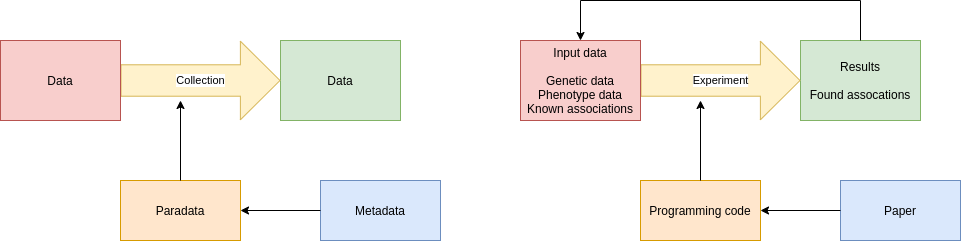
\includegraphics[width=\linewidth]{figure_1.png}
  \caption{
    \textbf{Left}: general relation between data, paradata and metadata.
    \textbf{Right}: the same relations specified for genetic epidemiology.
    Input data: genetic data, phenotypic data and associations
    found in earlier studies.
    Results: associations between genetic data and phenotypic data.
    Code: the computer code used in a computational experiment
    Paper: the scholarly paper describing the (code of the) experiment
  }
  \label{fig:figure_1}
\end{figure}

%%%%%%%%%%%%%%%%%%%%%%%%%%%%%%%%%%%%%%%%%%%%%%%%%%%%%%%%%%%%%%%%%%%%%%%%%%%%%%%%
\section{Code availability}\label{sec:code-availability}
%%%%%%%%%%%%%%%%%%%%%%%%%%%%%%%%%%%%%%%%%%%%%%%%%%%%%%%%%%%%%%%%%%%%%%%%%%%%%%%%

To determine how useful code is, it needs to be available.
However, it is not common to publish the code of an experiment or analysis 
(\cite{stodden2011trust,read2015sizing}) (with a pleasant exception 
being \cite{conesa2019making}).
For example, in computer graphics, 
a field intimately familiar with computer code,
42\% of 454 SIGGRAPH papers supply computer code (\cite{bonneel2020code}).
Another study analysed the reproducibility of registered reports
in the field of psychology, 
where 60\% of 62 studies supplied the code 
to redo the analysis (\cite{obels2020analysis}).
For articles in Science magazine, 12\% of 204
studies published the code (\cite{stodden2018empirical}) 
(note that these were years 2011-2012).
Unpublished code has been the cause of some saddening examples,
such as an algorithm that detects breast cancer from images 
better than a human expert, 
yet failed to ever be reproduced (\cite{haibe2020importance}).

% \paragraph{Obtaining code by email}

When code of an academic paper is not published, 
one could contact the corresponding author and request it.
However, the response rate of corresponding authors 
with a request for data in computational fields is around 50\% 
(\cite{manca2018non, stodden2018empirical, teunis2015corresponding}) 
(the field of emergency medicine seems to be a pleasant outlier, 
with 73\% of 118 emails being replied (\cite{o2003email})).
When getting an answer of the corresponding author, 
48\% out of 134 replied emails will actually result 
in a sharing of the code (\cite{stodden2018empirical}).
The responses of unwilling authors (see \cite{stodden2018empirical} for 
some real examples) can come across as so caustic, 
that one may be excused from not contacting an a corresponding author.

%%%%%%%%%%%%%%%%%%%%%%%%%%%%%%%%%%%%%%%%%%%%%%%%%%%%%%%%%%%%%%%%%%%%%%%%%%%%%%%%
\section{Genetic epidemiology}
%%%%%%%%%%%%%%%%%%%%%%%%%%%%%%%%%%%%%%%%%%%%%%%%%%%%%%%%%%%%%%%%%%%%%%%%%%%%%%%%

% \paragraph{Introduction}

This paper uses genetic epidemiology as a specific example,
to illustrate in which way code is paradata,
and why this type of paradata is relevant.
However, any field that uses computation 
and sensitive data in its experiments,
could be used as an example.

% \paragraph{For some fields, the experiment is actually run by code}

Genetic epidemiology is a field within biology that
tries to determine the spread of heritable traits 
and their underlying biological mechanism.
For example, we know that lactose intolerance in adults is
caused by a decline in the production of lactose-degrading enzymes,
and is most commonly found in south-east Asia and south 
Africa (\cite{storhaug2017country}).
The trait is caused by the genetic make-up, or 'genotype'
\iffalse
(see Table \ref{tab:definitions} in the Supplementary Materials
for the definitions of terms used in this paper)
\fi
, of a person.
The trait, also called 'phenotype', 
in this example is lactose intolerance at adult age,
yet any human property, such as weight or height can be studied.
When an association between genotype and phenotype is found,
these associations, when relevant enough, are used to 
create so-called 'gene panels', 
where the location of the gene causing 
an association is measured specifically, 
to detect people at risk for the associated phenotype.
The rest of this section describes a genetic epidemiology study 
in more detail, with special focus on the computational experiment.

\iffalse
\begin{figure}[!htbp]
  \centering
  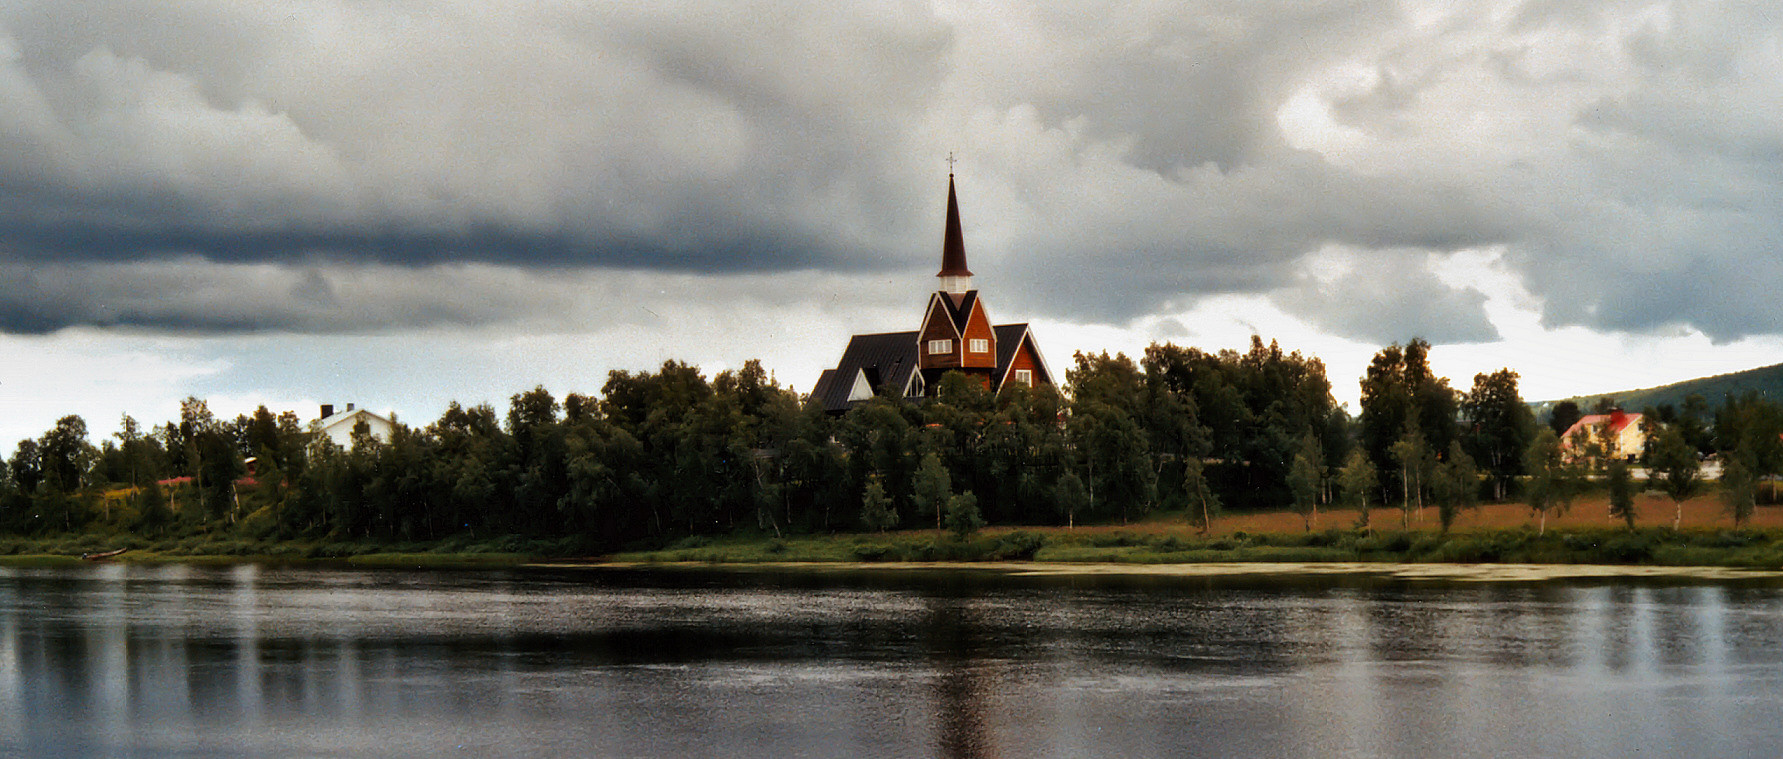
\includegraphics[width=\linewidth]{Karesuando_church.jpg}
  \caption{
    Picture of Karesuando's church,
    the village where the Northern Swedish Population
    Health Study started.
    From \cite{hopfner2005}
  }
  \label{fig:karesuando_church}
\end{figure}
\fi

The example study followed is a pseudorandomly selected paper
from \cite{ahsan2017relative}. The primary data used by that paper is
from a population study called the Northern Swedish Population
Health Study (NSPHS) that started in 2010 (\cite{igl2010northern}). 
The approximately 1000 participants were initially mostly surveyed
about lifestyle (\cite{igl2010northern}) and follow-up studies
provided the type of data relevant for this paper, 
which are (1) the genotypes (\cite{johansson2013identification}),
(2) the phenotypes, in this case, concentrations of certain proteins in the 
blood (\cite{enroth2014strong,enroth2015effect}).

\iffalse
\begin{figure}[!htbp]
  \centering
  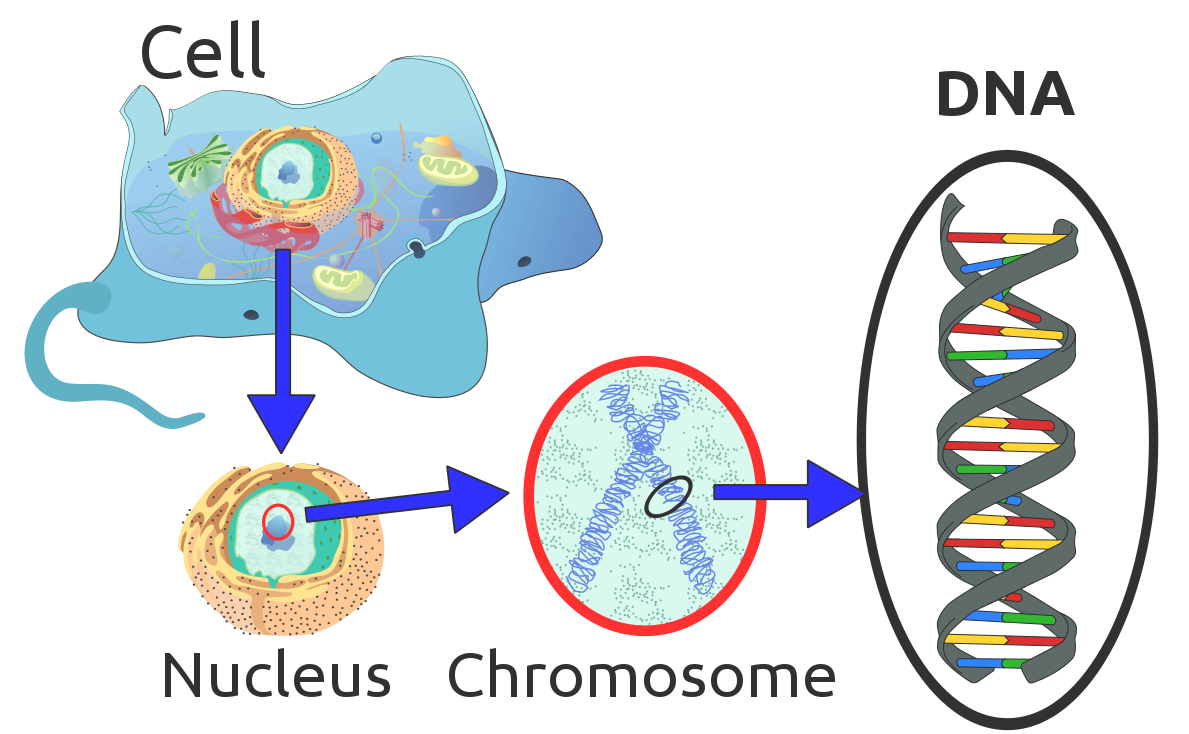
\includegraphics[width=\linewidth]{1189px-Eukaryote_DNA-en.png}
  \caption{
    A cell has a nucleus that contains chromosomes. 
    Each of these chromosomes (46 in humans) consist out of DNA. 
    DNA itself consists out of 4 nucleotides, 
    as depicted by the horizontal sticks 
    with the colours red, yellow, green and blue.
    From \cite{sponk2012}
  }
  \label{fig:eukakyote_dna}
\end{figure}
\fi

The first type of primary data, the genotypes, 
consists out of single nucleotide polymorphisms (SNPs, pronounced 'snips').
A SNP has a name and a location within the genome.
At the SNP's location in the DNA, there will be two nucleotides.
One of these nucleotides is inherited from the mother, 
the other from the father.
The DNA consists out of billions of nucleotides.
There are four types of nucleotides,
called adenosine, cytosine, guanine and thyrosine, 
commonly abbreviated as A, C, G and T 
\iffalse
(see figure \ref{fig:eukakyote_dna}))
\fi
respectively.


One SNP example is \verb|rs12133641|, which is a SNP located at position 
154,428,283 (that is, at the 154 millionth nucleotide), 
where 67 percent of the people within this study have an A,
and 33 percent have a G (also from \cite{ahsan2017relative}, Table S3).
From this it follow (assuming the nucleotides are inherited independently)
that 45\% of subjects have the genotype AA, 44\% have AG and 11\% have GG.

\iffalse
\begin{figure}[!htbp]
  \centering
  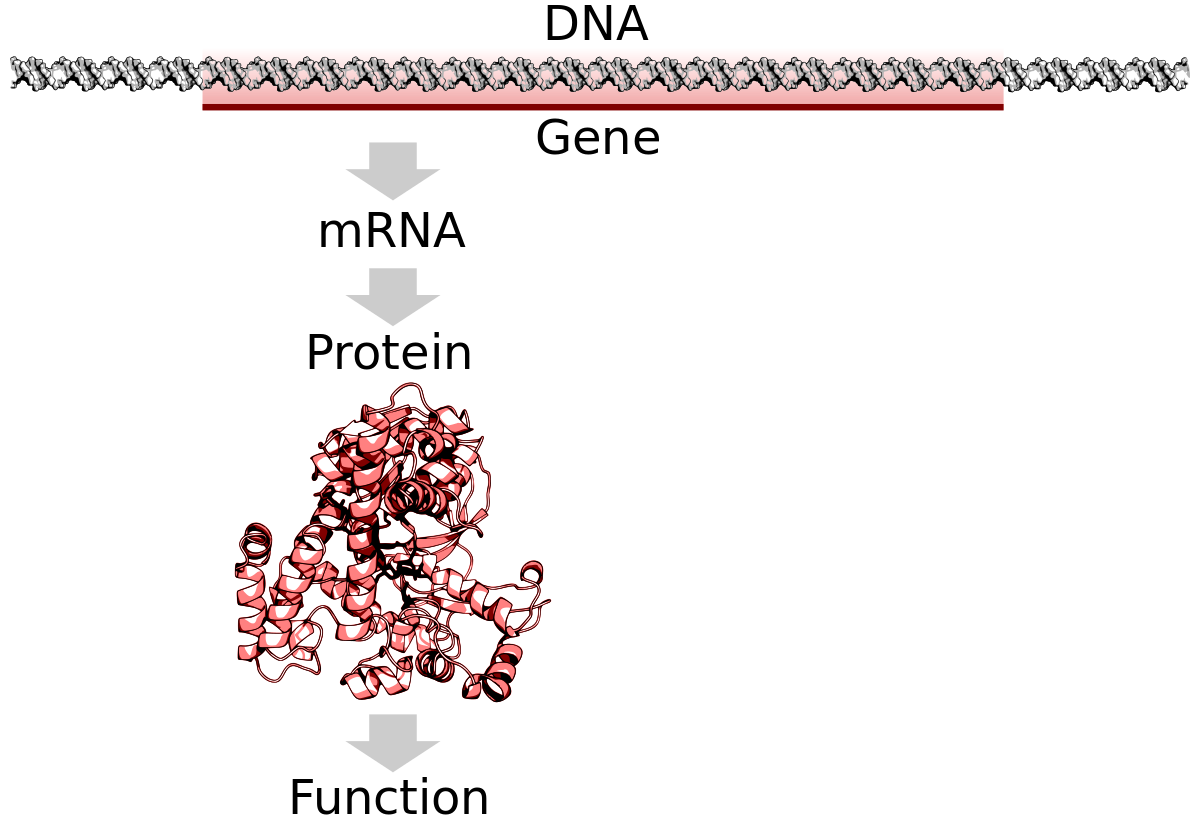
\includegraphics[width=\linewidth]{DNA_to_protein.png}
  \caption{
    Parts of DNA (so-called 'genes') code for proteins. 
    The DNA, that always stays put in the cell's nucleus, 
    is transcripted to messenger RNA (mRNA).
    mRNA leaves the nucleus and its code gets translated to 
    a protein sequence.
    Near the start of a gene are regions that determine the amount
    of proteins produced (not shown in figure).
    Adapted from \cite{shafee2015}
  }
  \label{fig:dna_to_protein}
\end{figure}
\fi

The second type of data, the phenotypes, 
are concentrations of proteins in the blood. 
The nucleotides of the DNA contain the code for building proteins
\iffalse
(see Figure \ref{fig:dna_to_protein})
\fi
,
as well as the rate at which a protein is created (for 
sake of simplicity it is assumed that such a rate is constant,
yet, in practice there are complex regulation mechanisms).
Some proteins end up in the blood and
their presence can be used to assess the health of an individual.
IL6RA is one such protein and its concentration may (and will, see below)
be associated with the SNP mentioned earlier.

The field of genetic epidemiology looks -among others- for
correlations between genetic data and biological traits.
For example, Ahsan and colleagues show that
SNP \verb|rs12133641| is highly correlated (p-value is $3.0^{-73}$
\iffalse
(see figure \ref{fig:ahsan2017relative_table_2_sub})
\fi
,
for $n$ = 961 individuals) with protein IL6RA (\cite{ahsan2017relative}).
The direction of the association is also concluded:
the more guanines are present at that SNPs location,
the higher concentration of IL6RA can be found in a human's blood
\iffalse
(see figure \ref{fig:ahsan2017relative_table_2_sub})
\fi
. The amount of variance that can be explained by an association (i.e.
the \begin{math}R^2\end{math}) is rarely 100\%, which means that a trait (in
this case, the concentration of IL6RA) cannot be perfectly explained
from the genotype (in this case, SNP \verb|rs12133641|) alone. 
In this example, as much as 43\% of the variance 
can be attributed to an individuals' genotype
\iffalse
(see figure \ref{fig:ahsan2017relative_table_2_sub})
\fi
. Additional factors, 
such as the effect
of the environment (e.g. geographic location, time of day the measurement 
was done), lifestyle (e.g. smoking yes/no) or having a disease (e.g. diabetes) 
are needed to explain the additional variation.

\iffalse
\begin{figure}[!htbp]
  \centering
  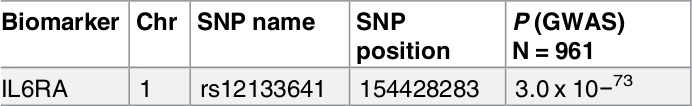
\includegraphics[width=\linewidth]{ahsan2017relative_table_2_sub.png}
  \caption{
    An example result of a genetic epidemiological research.
    It shows that the SNP named rs12133641 (located at position 154,428,283
    of chromosome 1) is highly correlated (p value is 3.0 * 10e-73, 
    961 individuals) to the concentration of the protein IL6RA, as measured
    in blood. The table is a simplified result from \cite{ahsan2017relative}.
  }
  \label{fig:ahsan2017relative_table_2_sub}
\end{figure}
\fi

\iffalse
\begin{figure}[!htbp]
  \centering
  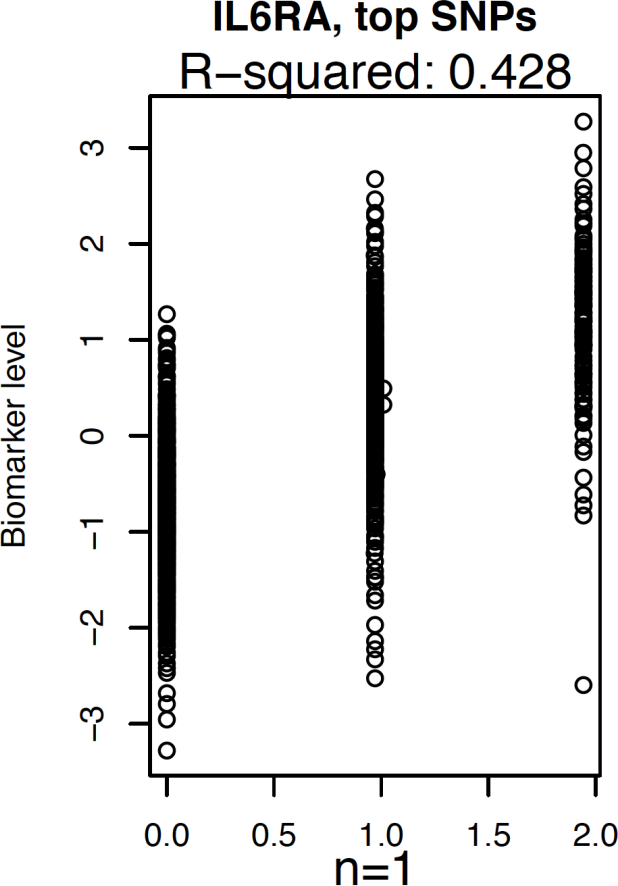
\includegraphics[width=\linewidth]{ahsan2017relative_s6.png}
  \caption{
    The relation between the genotype for SNP rs12133641 
    and the protein concentration of IL6RA is relatively strong.
    The X axis shows the the genotype of the individuals,
    where 0 denotes AA, 1.0 denotes AG and 2.0 denotes GG.
    The Y axis shows the concentration of the protein IL6RA 
    as found in the participants' blood. n = 1 denotes the number
    of SNPs that were determined to be involved.
  }
  \label{fig:ahsan2017relative_s6}
\end{figure}
\fi

The conclusions drawn from this paper,
may end up in the clinic.
For the sake of having a clear (yet fictitious) example,
let's assume that a high level of IL6RA 
is associated with a disease that develops later in life,
yet is preventable by lifestyle 
changes (see \cite{pope2003will} for an example in Alzheimer's disease).
Would this be the case, we can create a tailored 
experiment, called a gene panel, that specifically measures
SNP \verb|rs12133641|. 
If the gene panel shows an individual has two guanines, 
we know that this person is likelier to develop higher levels of
IL6RA and is likelier to benefit from the lifestyle changes.

From this simple example, it will be easier
to measure the level of IL6RA in the blood, than using a gene panel,
as blood tests are easier and cheaper.
However, there are associations published for many diseases,
in which one SNP (e.g. phenylketonuria) or many SNPs (e.g. \cite{bruce2009metabolic}) 
contribute to being more likely to develop a disease in the future. 
Here, the phenotype (having a disease in the future) 
is impossible to detect at the present
and associations found in earlier studies are used to create a gene panel.
As creating a gene panel is costly, those associations better be correct.

Additionally, there is an interdependency of scholarly findings here:
the SNP has received its name based on a computational experiment.
This earlier experiment that concluded the usefulness of that SNP, 
is based on some DNA sequences.
This experiment is based on assumed DNA sequences.
DNA sequences, however, are (nowadays) not simply read, 
yet are the result of a complex computational analysis instead,
with its own dedicated field of research.
Both studies assumed a correctly calculated DNA sequence.
This means that if the DNA sequence analysis contained a software bug, 
this study may be invalidated. 
Additionally, the result of this study may be used in follow-up studies,
that assume the result to be correctly calculated: one paper's conclusion
is the next paper's assumption.

%%%%%%%%%%%%%%%%%%%%%%%%%%%%%%%%%%%%%%%%%%%%%%%%%%%%%%%%%%%%%%%%%%%%%%%%%%%%%%%%
\section{Why code is useful paradata}
%%%%%%%%%%%%%%%%%%%%%%%%%%%%%%%%%%%%%%%%%%%%%%%%%%%%%%%%%%%%%%%%%%%%%%%%%%%%%%%%

% \paragraph{The experiments within genetic epidemology works are done by code}

The experiment described above is run by code. 
It was code that detected the relationship between the genotype
(in this case, SNP \verb|rs12133641|) 
and the phenotype (in this case, the concentration of IL6RA).
To be more precise, it was code that read the data,
subsetted the data, removed outliers, 
performed the statistics and generated the plots.
For the rest of the discussion, we assume that the
code is available to us (if not, see section \ref{sec:code-availability} 
for a glum estimate of the chance of obtaining the code).

% \paragraph{Why useful code}

There are multiple reasons why (useful) code matters,
and these are the same reasons as why useful paradata matters:
code gives an understanding how the raw results 
and the subsequent scholarly knowledge is obtained from an experiment.
Additionally, code helps researchers from different fields 
to understand each other and collaborate.
Additionally, code helps Open Science reach its goals of openness and
transparency.
The core of these reasons it to achieve reproducible science:
that any person in any field can redo a computational experiment
and see exactly what happened.

% \paragraph{The goal of useful paradata is reproducible science}

For computational science, it may appear to be relatively easy to 
reproduce an experiment, as all it takes is a computer, electricity,
an optional internet connection, the code and the data.
In practice, however, 
only 18\% of 180 computational studies 
are easily reproducible (\cite{stodden2018empirical}).
To some, it appears that 
the academic culture to reproduce results 
has been lost over time \cite{peng2011reproducible},
with labs that embrace reproducibility (for example, \cite{barba2016hard})
being the exception.
One suggested way forward is to make the reproduction of 
research a minimal requirement for publication (\cite{peng2011reproducible}).

% \paragraph{Sensitive data}

A genetic epidemiologist works with sensitive data as well:
the genetic sequences of participants are private (\cite{clayton2019law}).
For research to be reproducible one needs both the code and the data
to reproduce the (hopefully) same results.
This problem is discussed in section \ref{sec:sensitive-data}.

% \paragraph{Code holds the ground truth}

\iffalse
\begin{figure}[!htbp]
  \centering
  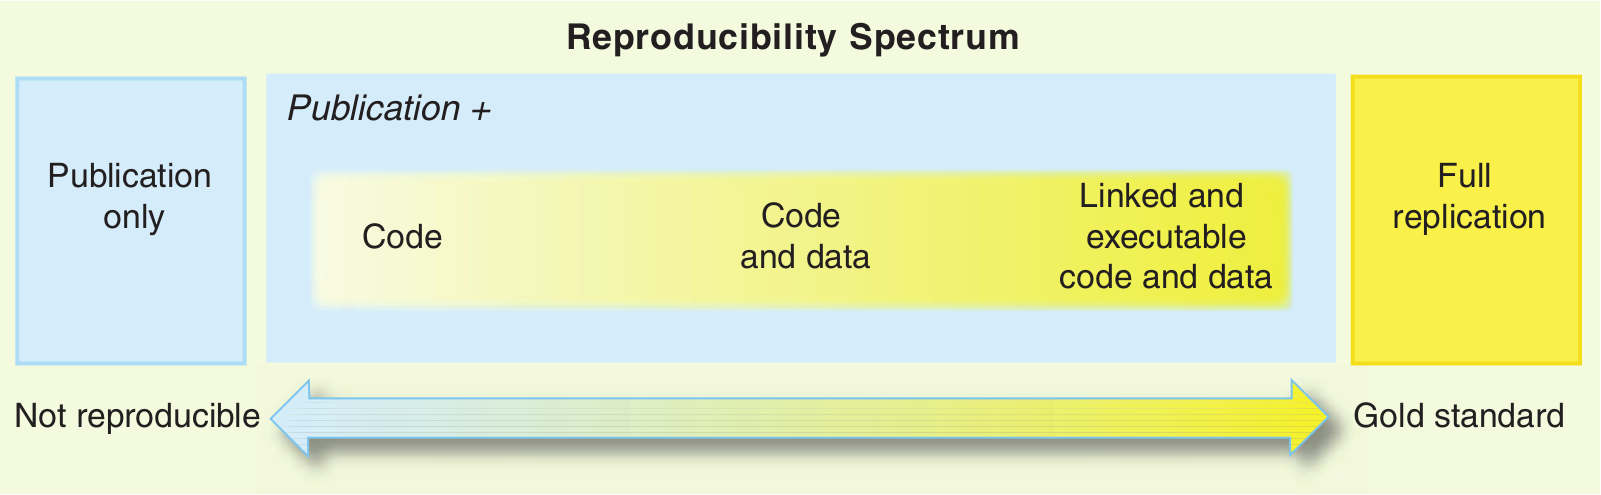
\includegraphics[width=\linewidth]{peng2011reproducible_fig_1.png}
  \caption{
    Levels of reproducibility, from \cite{peng2011reproducible}
  }
  \label{fig:peng2011reproducible}
\end{figure}
\fi

\iffalse
To illustrate how easy it is to get a mismatch between a paper
and the code, 
consider this example of a possible text in the fictional 
genetic epidemiology paper:

\textit{
  We compared the in-blood concentrations of IL6RA 
  between subjects having AA versus subjects having GG at SNP rs12133641,
  using an unpaired one-tailed T-test,
  as we expect the average concentration of IL6RA for those with AA 
  to be less than the average concentration in those with GG.
}

We ignore the choices of words and style of this sentence: what is
important is the content: an unpaired one-tailed T test is performed.
Taking a look at the (in this case, the programming language R (\cite{r})) code, 
we find the following line:

\begin{verbatim}
t_test_result <- t.test(subjects_with_aa, subjects_with_gg)
\end{verbatim}

The code is correct:
\verb|t.test| is indeed the name of an R function to do an unpaired T-test
and it is reasonable to assume that this code, when glancing over the code
of an article, is correct.

Here, however, we see a mismatch between the English description and the code:
by default, the R function \verb|t.test| does 
a \textbf{two}-tailed unpaired T-test.
A consequence of this fictional example is that the published p-values are
higher than needed, resulting in less significant findings, which
results in (needlessly) less conclusions drawn in this fictional paper.

Note that there is another side of this same coin:
correctly reporting the t-test in a reproducible ways
is known to be a problem, with only 80 out of a selected 179 papers
fully reporting the parity of t-test (i.e. paired or unpaired) 
(\cite{weissgerber2018we}).
In those unresolved 99 papers, 
the code (if published) would clarify this.
\fi

\iffalse
\begin{figure}[!htbp]
  \centering
  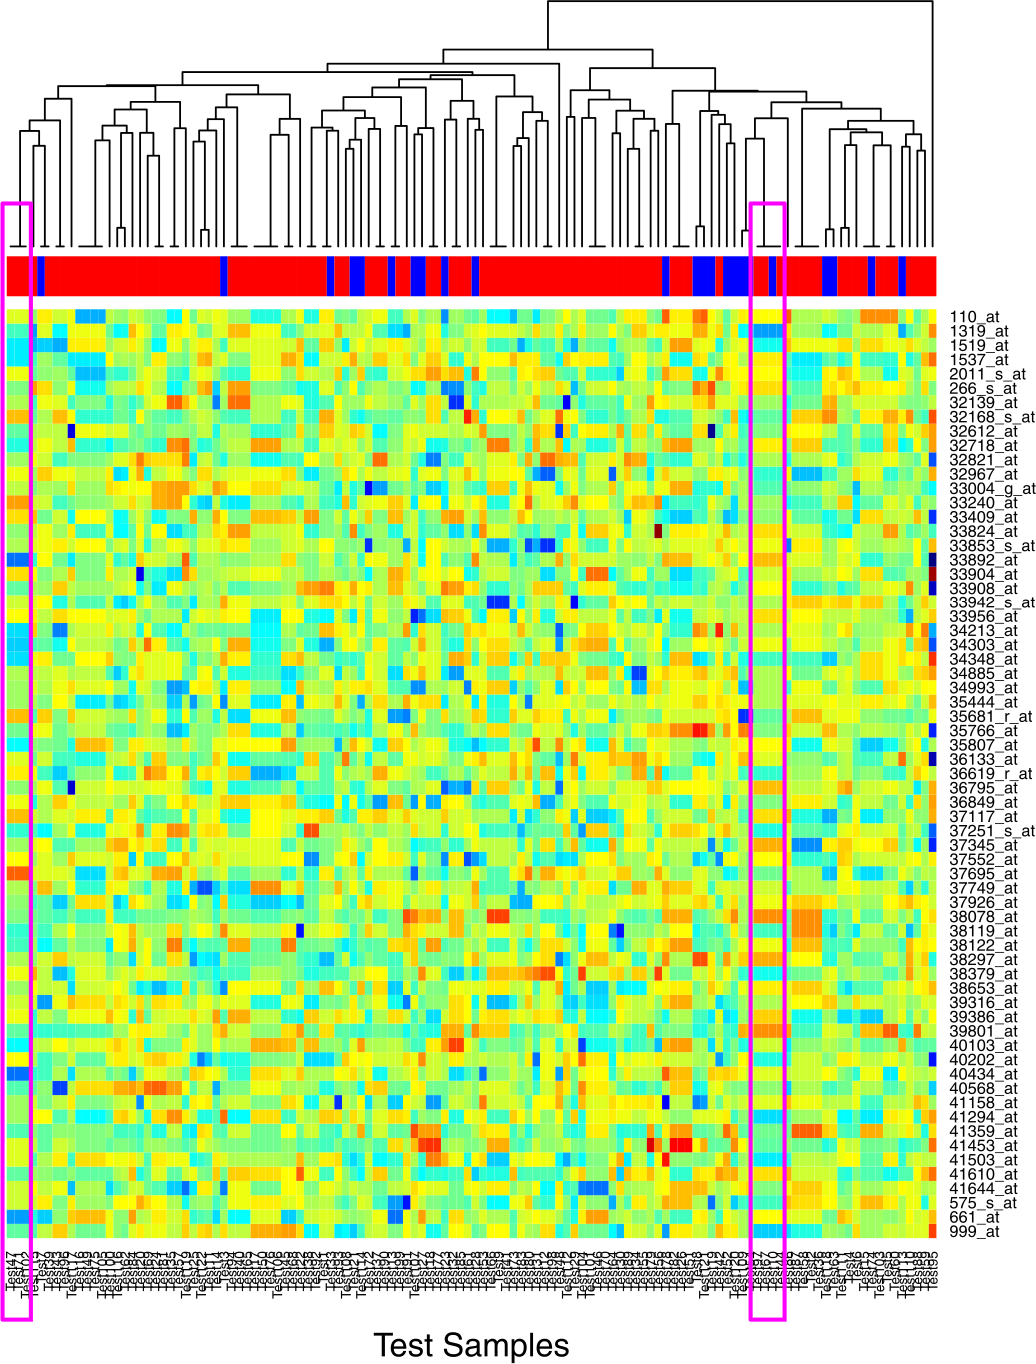
\includegraphics[width=\linewidth]{baggerly2009deriving_fig_1a.png}
  \caption{
    Gene expression result due to an off-by-one error.
    The cells in the main table show how much mRNA is produced per cell 
    line (the columns) for different proteins (the rows).
    The colours above the cells, with the dendrogram, shows
    red for cells that do not respond (red) and do respond (blue) to an 
    antibiotic.
    The purple rectangles show samples that are duplicated.
    Note that, due to this, some
    samples that behave identically are both non-responders and responders.
    From \cite{baggerly2009deriving}
  }
  \label{fig:baggerly2009deriving}
\end{figure}
\fi

Code holds the ground truth of an experiment; it does the actual work.
The more complex the computation pipeline is, the easier it is
to have a mismatch between the article (that describes what the
code does) and the code (that actually does the work).
The moment these two disagree, it is the code that is true.

%%%%%%%%%%%%%%%%%%%%%%%%%%%%%%%%%%%%%%%%%%%%%%%%%%%%%%%%%%%%%%%%%%%%%%%%%%%%%%%%
\section{Preserving code}
%%%%%%%%%%%%%%%%%%%%%%%%%%%%%%%%%%%%%%%%%%%%%%%%%%%%%%%%%%%%%%%%%%%%%%%%%%%%%%%%

Code is rarely preserved (\cite{barnes2010publish}).
This section discusses the preservation of code for a short, medium
and long term.

\subsection{Code hosting}\label{subsec:code-hosting}

To preserve code for a short term, 
a code hosting website is a good first step.
A code hosting website is a website where 
its users can create dedicated pages (called 'repositories')
for a project, upload code and interact with that code.
There are multiple code hosting websites, 
with GitHub being the most popular one (\cite{cosentino2017systematic}).
The use of code hosting websites
has increased strongly (\cite{russell2018large}),
accommodates collaboration (\cite{perez2016ten})
and improves transparency (\cite{gorgolewski2016practical}),
due to its inherent computer-friendliness.
See \cite{cosentino2017systematic} for an extensive overview of
research conducted on GitHub.

\iffalse
An example from the author is the website (\cite{bbbqarticleissue157}),
that hosts part of the code for the paper \cite{bilderbeek2022transmembrane}, 
as shown in Figure \ref{fig:bbbqarticleissue157}.
Also, the \LaTeX \hspace{5mm} code of this chapter is hosted on GitHub 
as well, at \url{https://github.com/richelbilderbeek/chapter_paradata}.
\fi

\iffalse
\begin{figure}[!htbp]
  \centering
  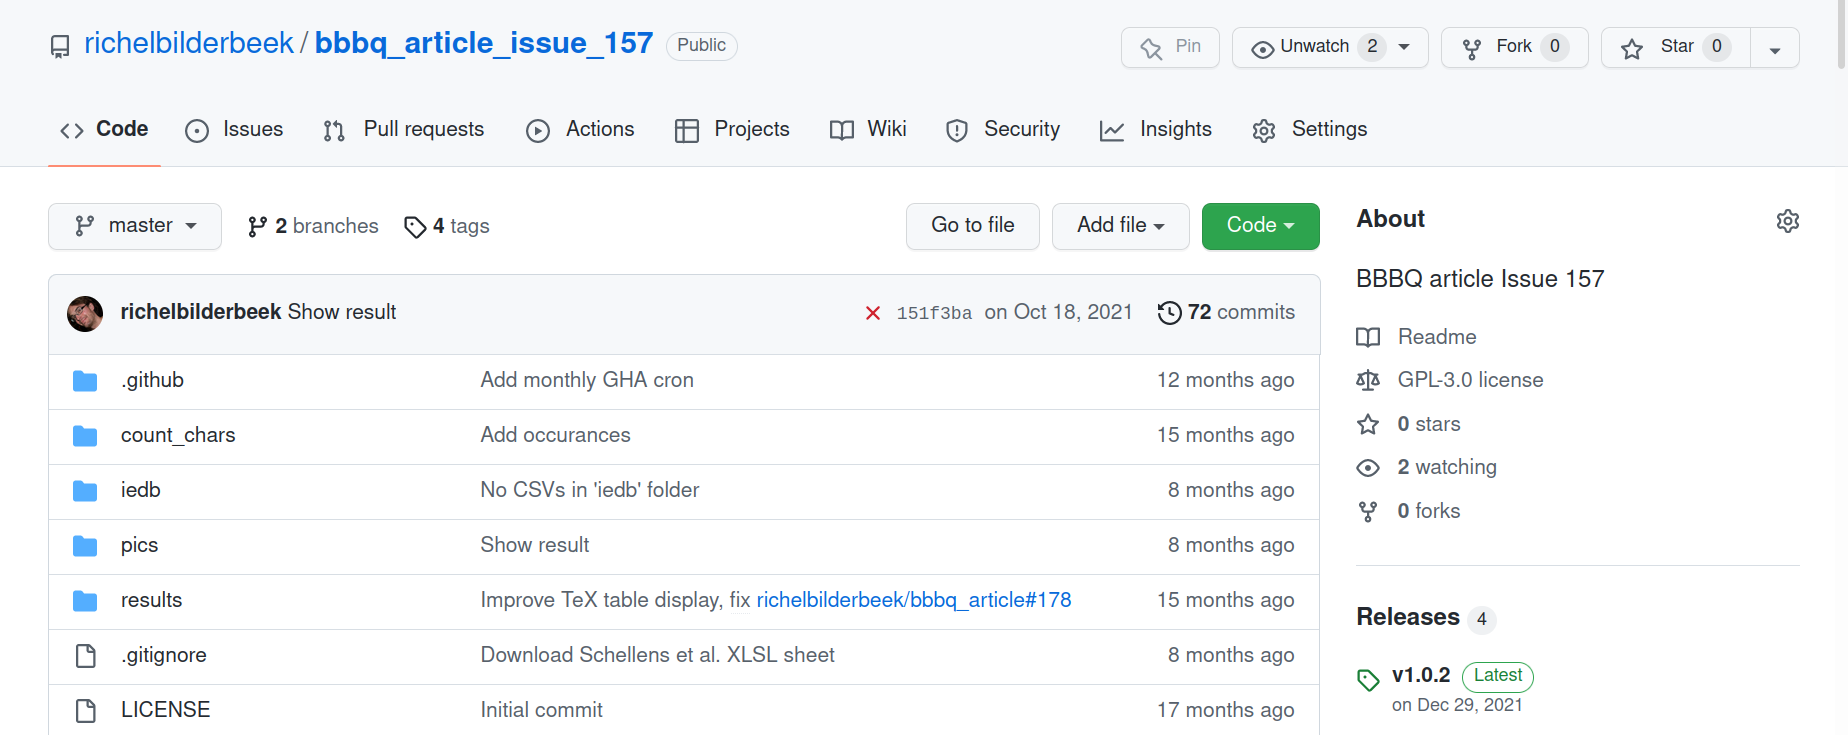
\includegraphics[width=\linewidth]{bbbq_article_issue_157.png}
  \caption{
    A typical GitHub repository \cite{bbbqarticleissue157}, 
    hosting the code for a
    computational experiment, 
    as published with \cite{bilderbeek2022transmembrane}.
    Note that this repository has 72 commits, where a commit is a change
    to the code.
  }
  \label{fig:bbbqarticleissue157}
\end{figure}
\fi

% \paragraph{Hosted code keeps a history of changes}

Hosted code commonly keeps a history of file changes,
This means that when a change is made to the code,
a new version is created. In the case that the change was harmful,
one can go back to an earlier version and continue again from there.
The version control system keeps track of who-did-what transparantly.
\iffalse
Figure \ref{fig:daisie_contributors}
shows the number of commits the authors of DAISIE (\cite{etienne2020daisie})
have made to its code.
\fi
It is a general recommendation to put version control
on all human-produced data (\cite{wilson2014best}),
as well as openly working on the code from the start (\cite{jimenez2017four}).
Half of the published code has such a version control 
system (\cite{stodden2018empirical}).

\iffalse
\begin{figure}[!htbp]
  \centering
  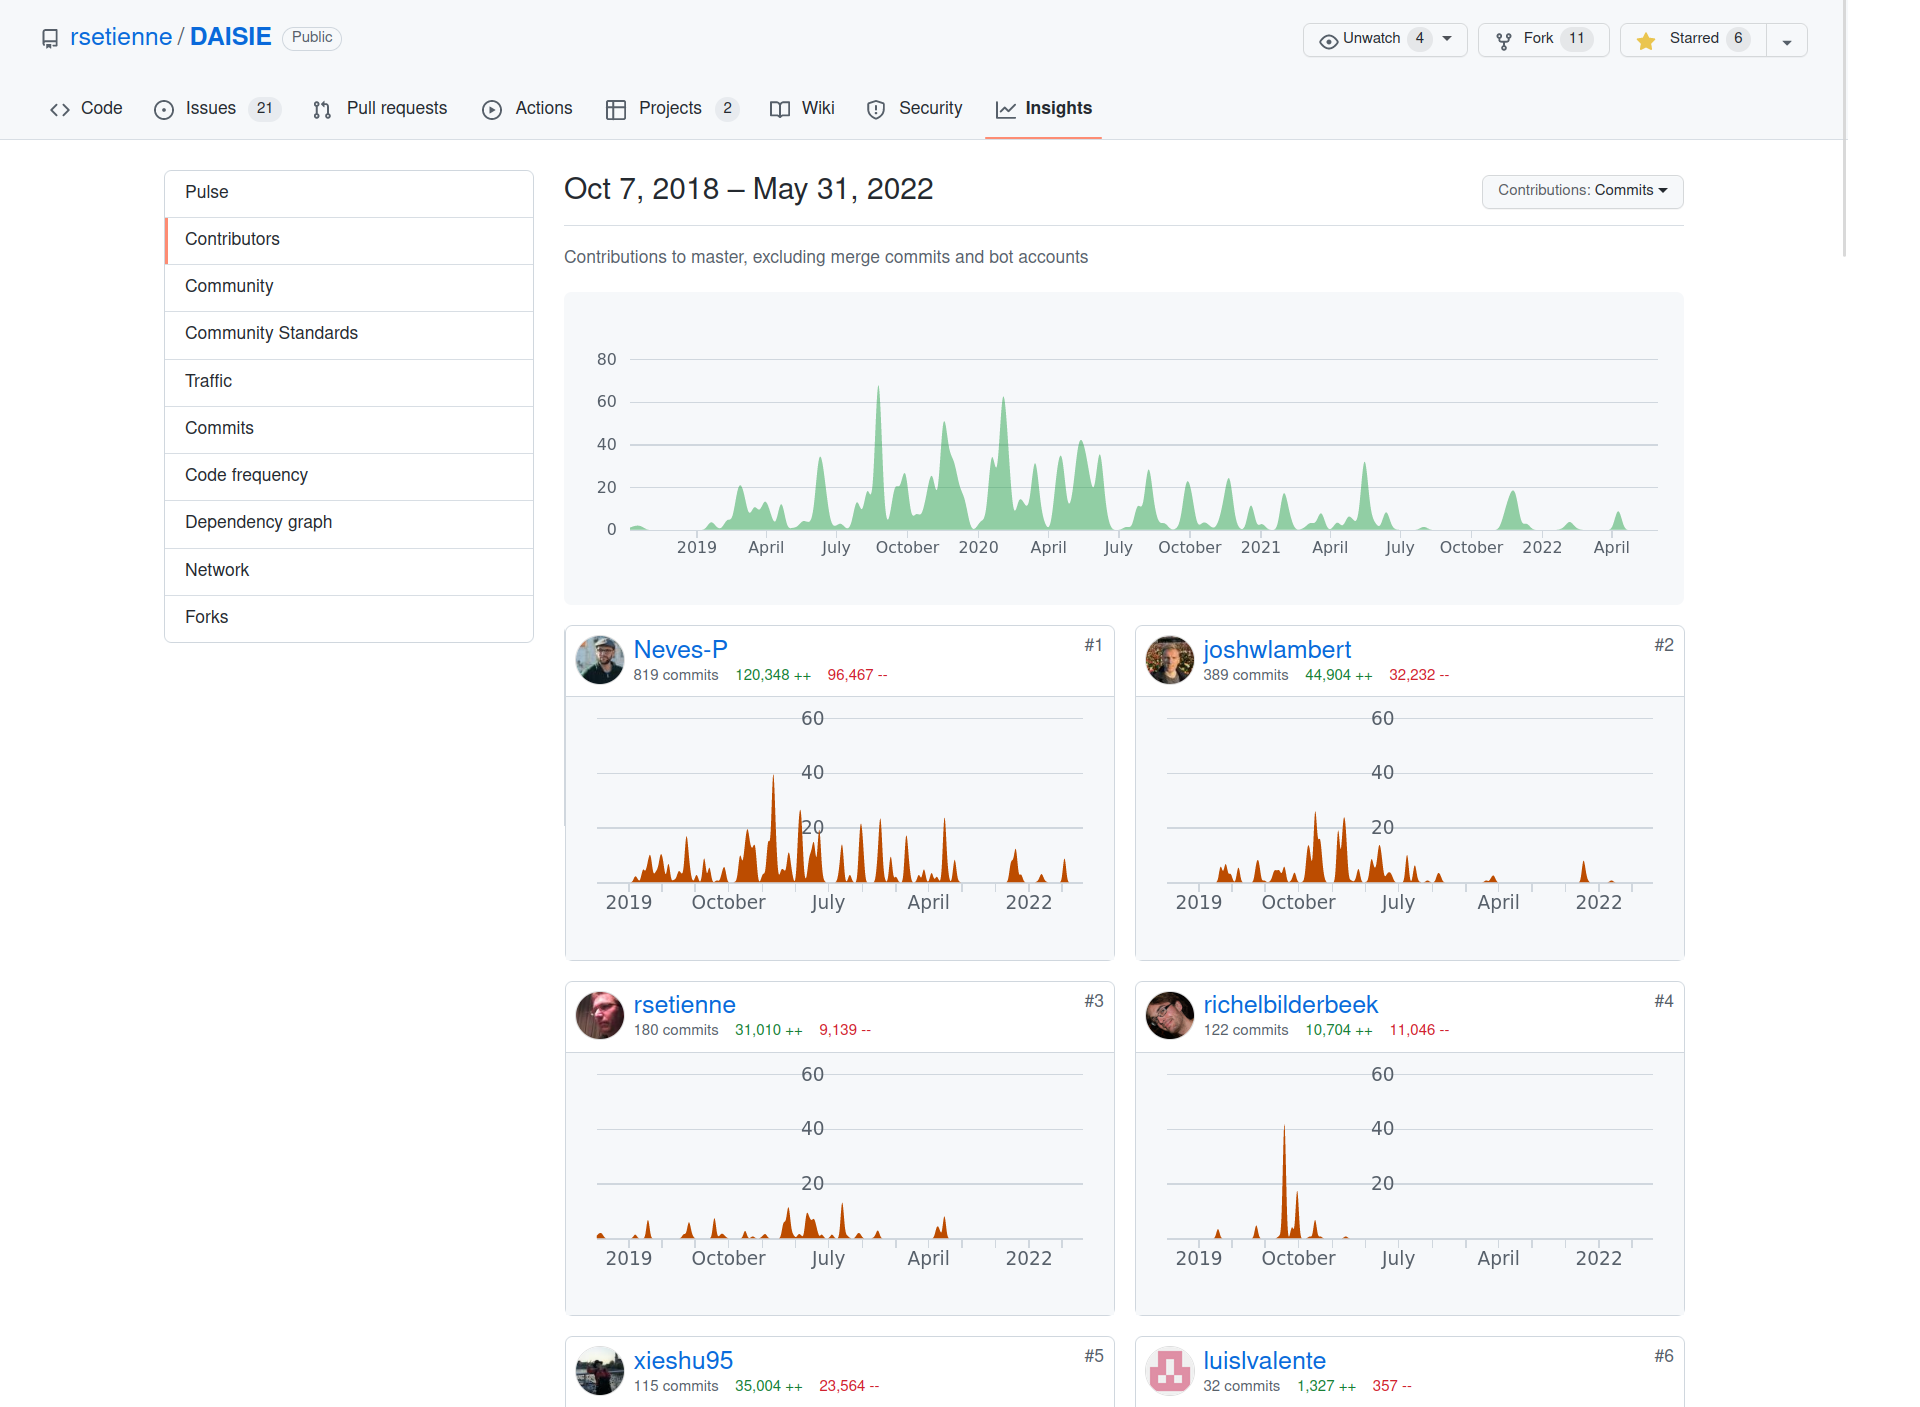
\includegraphics[width=\linewidth]{daisie_contributors.png}
  \caption{
    An overview of the commits that multiple contributors have
    made, in this case, to the code of DAISIE \cite{etienne2020daisie}
  }
  \label{fig:daisie_contributors}
\end{figure}
\fi


The degradation of software is a known feature for nearly 
four decades.
This is called 'bit rot' by \cite{steele1983hacker},
or 'software collapse' by \cite{hinsen2019dealing},
in which software fails due to dependencies on other 
software.
Using a code hosting website, 
that only passively stores code,
ignores this problem.

\subsection{Continuous integration}

To preserve code for a longer timespan, 
it needs to be embraced that software degrades (\cite{beck2000extreme}).
Continuous integration ('CI') allows one to 
verify if code still works and, if not, to be notified.

% \paragraph{Continuous integration helps assess code quality}

Some code hosts,
allow a user to trigger specialised code upon uploading a change,
called a CI script.
Such a CI script typically builds and tests the code.
This practice is known to significantly 
increase the number of bugs exposed (\cite{vasilescu2015}) and increases
the speed at which new features are added (\cite{vasilescu2015}).
CI can be scheduled to run on a regular basis and
notify the user directly when the code has broken down.

\subsection{Containerisation}

To preserve code for the longest time, 
both code and its dependencies can be put into a so-called container.

The most reproducible way of submitting the code of an experiment,
is to put all code with all the (software) dependencies
in a file that acts as a virtual computational environment,
called a 'virtual container' (from now on: 'container').
Such a container is close to the golden standard of reproducible research
as suggested by 
\cite{peng2011reproducible} 
\iffalse
(see also Figure \ref{fig:peng2011reproducible})
\fi
.

%%%%%%%%%%%%%%%%%%%%%%%%%%%%%%%%%%%%%%%%%%%%%%%%%%%%%%%%%%%%%%%%%%%%%%%%%%%%%%%%
\section{Making code useful paradata}\label{sec:making-code-useful-paradata}
%%%%%%%%%%%%%%%%%%%%%%%%%%%%%%%%%%%%%%%%%%%%%%%%%%%%%%%%%%%%%%%%%%%%%%%%%%%%%%%%

Useful paradata, in general, are (1) comprehensive,
(2) documented appropriately, (3) documented in co-evolution with the data,
and (4) friendly to computers (\cite{huvila2022improving}).
In this section, these ideal properties of paradata are applied to code.

However, code has multiple uses,
as code can be used to (1) reproduce, (2) replicate, or (3)
extend a computational experiment (\cite{benureau2018re}).
Depending on the intended use of the code,
there are different requirements for code being useful paradata.

%%%%%%%%%%%%%%%%%%%%%%%%%%%%%%%%%%%%%%%%%%%%%%%%%%%%%%%%%%%%%%%%%%%%%%%%%%%%%%%%
\subsection{Code must be usefully documented}
%%%%%%%%%%%%%%%%%%%%%%%%%%%%%%%%%%%%%%%%%%%%%%%%%%%%%%%%%%%%%%%%%%%%%%%%%%%%%%%%

For code to be ideal paradata, it must be usefully 
documented (\cite{huvila2022improving}).

For purposes of reproducing code,
it should at least be documented how to run the code and what it ought to do.
Although this may be obvious, only 57\% out of 56 Science papers 
with obtainable code (in total there were 180 papers) 
do so (\cite{stodden2018empirical}).

When it can be found out how how an experiment is run, 
it is possible (even ideal!) that no code is read at all.
Within that context, it could argued that no (further) documentation is needed.
However, all code in general should be documented 
'adequately' (\cite{peng2006reproducible}),
ideally writing code in such a way that it becomes 
self-explanatory (\cite{wilson2014best})
and for the remaining code to document the reasons behind it, 
its design and its purpose (\cite{wilson2014best}).

For purposes of extending a study and its code, 
documentation becomes even more important,
as the code will be read and modified.
The extent of investing time in documenting code is recommended
to be proportional to the intended reuse (\cite{pianosi2020successfully})
and there exists a clear relationship between the reuse 
of code and its documentation 
effort (\cite{cosentino2017systematic,hata2015characteristics}).

%%%%%%%%%%%%%%%%%%%%%%%%%%%%%%%%%%%%%%%%%%%%%%%%%%%%%%%%%%%%%%%%%%%%%%%%%%%%%%%%
\subsection{Code and documentation must align}
%%%%%%%%%%%%%%%%%%%%%%%%%%%%%%%%%%%%%%%%%%%%%%%%%%%%%%%%%%%%%%%%%%%%%%%%%%%%%%%%

For code to be ideal paradata, 
its creation and documentation need to align, 
\emph{not least because they shape each other} (\cite{huvila2022improving}).
This emphasised part of the quote resonates strongly with the idea of 
literate programming (\cite{knuth1984literate}),
in which documentation and code are developed hand-in-hand.
Literate programming is the practice of writing code and 
documentation in the same file.
Contemporary examples of this idea are, among others, 
vignettes (\cite{wickham2015r}) for the R programming language (\cite{r}) 
and Jupyter notebooks (\cite{wang2020assessing})
for the Julia (\cite{Julia-2017}), Python (\cite{van1995python}) and R (\cite{r})
programming languages.
rOpenSci, a community that, among others, reviews programming
code (\cite{ram2013ropensci,ram2018community}), is 
one example of where extensive documentation is mandatory
and all code must have examples (that are actually run)
as part of the documentation (\cite{ropensci_2021_6619350}).
In general, when developing software, 
it is recommended to 
to write documentation while writing software,
as well as to include many examples (\cite{lee2018ten}),
as this leads to both better code and documentation (\cite{reenskaug1989environment}).

%%%%%%%%%%%%%%%%%%%%%%%%%%%%%%%%%%%%%%%%%%%%%%%%%%%%%%%%%%%%%%%%%%%%%%%%%%%%%%%%
\subsection{Code must be extensive}
%%%%%%%%%%%%%%%%%%%%%%%%%%%%%%%%%%%%%%%%%%%%%%%%%%%%%%%%%%%%%%%%%%%%%%%%%%%%%%%%

For code to be ideal paradata, it must be extensive.
As code has many properties, there are many recommendations on this aspect.

% \paragraph{Code should be distributed in standard ways}

Code should be distributed in standard ways (\cite{peng2006reproducible}),
as is done by using a code hosting website
(see subsection \ref{subsec:code-hosting}).

% \paragraph{Code must have extensive error handling}

Code must be more extensive when it is (intended to be) 
used on different data,
as then 'code must act as a teacher for future developers' (\cite{sadowski2018modern}).
Error handling is one of the mechanisms to do so.
In genetic epidemiology, it is common to have incomplete or missing data,
so analyses should take this into account with clear error messages.

% \paragraph{Code must be tested}

Coding errors are extremely common (\cite{baggerly2009deriving, vable2021code})
and contribute to the reproducibility crisis in science (\cite{vable2021code}).
Testing, in general, is an important mechanism to ensure
the correctness of code.
One clear example is \cite{rahman2020exploratory}, 
showing bugs in scientific software on the COVID-19 pandemic.

% \paragraph{TDD}

Testing is so important that it is at the
heart of a software development methodology called 'Test-Driven 
Development' ('TDD'), in which tests are written
before the 'real' code.
TDD improves code quality (\cite{alkaoud2018quality,janzen2006test})
and it is easy to integrate 
the writing of documentation as part of the TDD cycle (\cite{shmerlin2015document}).

% \paragraph{Code coverage helps assess code quality}

The percentage of (lines of) code tested is called the code coverage.
Code coverage correlates with code quality (\cite{horgan1994,del1995correlation}).
and, due to this, having a code coverage of (around) 100\% 
is mandatory to pass a code peer-review
by rOpenSci (\cite{ram2018community}).
When CI is activated, 
the code coverage of a project can be shown on the repository's website
\iffalse
(e.g. as shown in Figure \ref{fig:badge_codecov})
\fi
.

\iffalse
\begin{figure}[!htbp]
  \centering
  
\includegraphics[]{badge_codecov.png}
  \caption{
    A build badge for the code coverage of an R 
    package (\url{https://github.com/ropensci/beautier}).
    The umbrella signals that the code coverage is hosted by
    CodeCov (\url{https://codecov.io/}). 
    The text indicates which process it is that the badge
    signals, which in this case, is that the code is fully covered
    by tests.
  }
  \label{fig:badge_codecov}
\end{figure}
\fi

\iffalse
CI opens up the possibility to informally annotate features of
a repository. 
For example, Figure \ref{fig:build_badge} shows a 
build badge that indicates that a \LaTeX document (i.e. this paper)
could be built.
\fi

\iffalse
\begin{figure}[!htbp]
  \centering
  
\includegraphics[width=\linewidth]{build_badge.png}
  \caption{
    A build badge for the GitHub repository of this article.
    The description indicates which process it is that the badge
    signals success (as in this case) or failure of. 
  }
  \label{fig:build_badge}
\end{figure}
\fi

% \paragraph{Adding a license}

It is considered good practice
to add a software license (\cite{jimenez2017four}),
so that it is clear that the software can be reused.
Although this may seem trivial, 
only two-thirds of 56 computational experiments 
supply a software license (\cite{stodden2018empirical}).

\iffalse
\begin{figure}[!htbp]
  \centering
  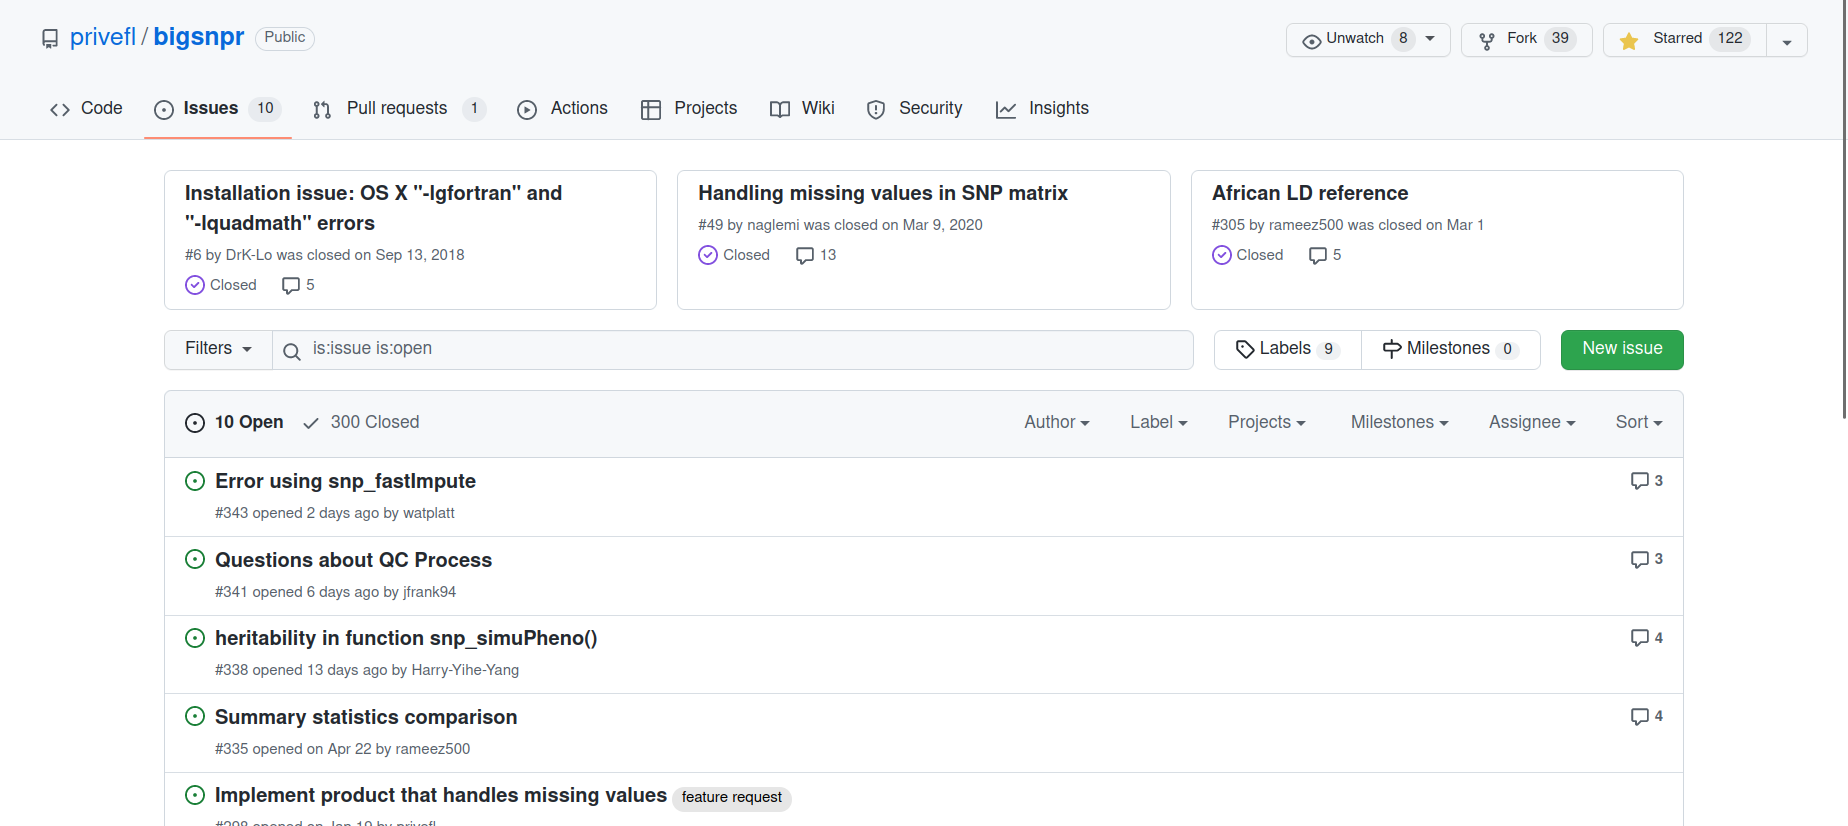
\includegraphics[width=\linewidth]{issue_ldpred2.png}
  \caption{
    An overview of the issues for the code for
    LDpred2 \cite{prive2020ldpred2}. Of the 310 issues, 300 have been closed.
    The first four issues have been replied to, as indicated by the
    talk balloon. The fifth issues has a label with the text 'feature request'
    to signal the issue type.
  }
  \label{fig:issue_ldpred2}
\end{figure}
\fi

% \paragraph{Code must be reviewed to ensure the correct amount of documentation}

Code reviews are recommended by software development 
best-practices (\cite{wilson2014best}).
However, more than half of 315 scientists 
have their code rarely or never reviewed (\cite{vable2021code}),
although code reviews are known to
accelerate learning of the developers,
improve the quality of the code
and resulting to an experiment that is likelier to be reproducible
(\cite{vable2021code}).

%%%%%%%%%%%%%%%%%%%%%%%%%%%%%%%%%%%%%%%%%%%%%%%%%%%%%%%%%%%%%%%%%%%%%%%%%%%%%%%%
\subsection{Code must be computer friendly}
%%%%%%%%%%%%%%%%%%%%%%%%%%%%%%%%%%%%%%%%%%%%%%%%%%%%%%%%%%%%%%%%%%%%%%%%%%%%%%%%

% \paragraph{Publishing a virtual environment}

The most reproducible way of submitting the code of an experiment,
is by providing the code with all its (software) dependencies 
in a container.

% \paragraph{Runnable code can precisely reproduce an experiment}

Containers allow a computation experiment to be highly reproducible:
given the same data, an experiment put into a container will give
the same results on different platforms, at least in theory.
In practice, differences may be observed when peripheral factors
are different, such as the random numbers as generated by an operating
system, or data that are downloaded from online (and hence, probably changing) sources.

% \paragraph{Ideal paradata}

For paradata to be useful, it has to be computer-friendly, yet 
'the best paradata does not necessarily look like 'data' at all for its
human users' \cite{huvila2022improving}.
There are features of code that humans find useful,
without directly being able to measure these.
In the end, code is just 'another kind of data' and should be designed 
as such, for example, by using tools to work on it (\cite{wilson2022twelve}).

% \paragraph{Using a tool for coding style}

A first example is to use a tool to enforce a coding style 
(e.g. the Tidyverse style guide (\cite{wickham2019advanced}) for R,
or PEP 8 (\cite{van2001pep}) for Python),
as following a consistent coding style improves software quality (\cite{fang2001}).

% \paragraph{Using a tool for complexity}

A second example is to use a tool to enforce a low cyclomatic complexity.
The cyclomatic complexity is approximately defined 
as the number of independent paths that
the code can be executed. 
\iffalse
For example, code that has only one \verb|if| statement
has a cyclomatic complexity of 2, as the condition within the \verb|if|
statement can be true or false,
resulting in the body of the \verb|if| statement being either
executed or ignored.
\fi
The cyclomatic complexity correlates with code complexity,
where more complex code is likelier to contain or give rise to bugs 
(\cite{abd2018calculating,chen2019empirical,zimmermann2008predicting}).

%%%%%%%%%%%%%%%%%%%%%%%%%%%%%%%%%%%%%%%%%%%%%%%%%%%%%%%%%%%%%%%%%%%%%%%%%%%
\section{Sensitive data}\label{sec:sensitive-data}
%%%%%%%%%%%%%%%%%%%%%%%%%%%%%%%%%%%%%%%%%%%%%%%%%%%%%%%%%%%%%%%%%%%%%%%%%%%

Next to the code, it is the data used in an experiment 
that must be made available for an experiment 
to be called 'reproducible' (\cite{peng2006reproducible}).
In some fields, such as genetic epidemiology, the data are
sensitive, hence cannot be released, thus one cannot reproduce 
an experiment.
To solve this problem in the future, there are some 
interesting methods being developed to run code on sensitive
data with assured privacy (\cite{zhang2016review,azencott2018machine}).

To alleviate the problem today,
a developer should supply a simulated 
(also called 'analytical' (\cite{peng2006reproducible})) dataset
together with the code.
This simulated data is needed to run tests, as is 
part of the TDD methodology.
In the case of genetic epidemiology this would mean
simulated genotypes and associated phenotypes,
as can be done with the \verb|plinkr| R package (\cite{plinkr}).
One extra benefit of simulated data is that these can be used
as a benchmark, as slightly different analyses should give 
similar conclusions.

%%%%%%%%%%%%%%%%%%%%%%%%%%%%%%%%%%%%%%%%%%%%%%%%%%%%%%%%%%%%%%%%%%%%%%%%%%%
\section{Discussion}
%%%%%%%%%%%%%%%%%%%%%%%%%%%%%%%%%%%%%%%%%%%%%%%%%%%%%%%%%%%%%%%%%%%%%%%%%%%

In a perfect world, all code has the characteristics of ideal paradata
and is written from software development best practices.
This section discusses the problems that arise by doing so.

% \paragraph{Invest in training}

To know these best practices, one needs to be trained. 
Articles that suggest these best practices (such as this one), 
claim that this initial investment pays off.
Code reviews are a good way to accelerate the 
learning of team members (\cite{vable2021code}).

% \paragraph{Code needs maintanance}

Code needs maintenance,
as code that will stand the test of time perfectly 
is deemed 'impossible' (\cite{benureau2018re}).
CI can help a maintainer to be notified when the code breaks,
where the use of containers may slow down time,
as an entire computational environment is preserved.

% \paragraph{Uploading code may feel like a risk}

Uploading code, preferably to a code hosting website, 
may feel like a risk, as all code can be seen and scrutinised.
However, not publishing code may put 
oneself in the focus of attention
and -after much effect by others reproducing an incorrect result-
at the cost of a scientific career (\cite{baggerly2009deriving}).

% \paragraph{Authors can be contacted}

When the author of code can be contacted,
there will be users asking for technical support 
(against which a 'no' is just fine (\cite{barnes2010publish}))
One solution for the author is to ignore such emails (as is done in a third
of all cases (\cite{teunis2015corresponding})):
it can be argued that no energy should be wasted on published code
and work on something new instead.
However, see \cite{barnes2010publish for a better way to deal with this problem.

% \paragraph{How to handle bugs?}

When the author of code can be contacted,
users will send in bug reports.
If the bug is severe enough, the question arises
if all the research that use that code still 
results in the same conclusions.
One such bug is described in \cite{eklund2016cluster},
with 40,000 studies using that incorrect code.
These reports could be ignored to work on something new.

% \paragraph{The problems with runnable code}

One problem that containers have, is their size:
they can be several gigabytes big. 
This makes the distribution of these containers harder.
Ideally, containers are stored online and distributed in
standardised ways.
Although progress is being made, 
there is no way to do so for all container types.
Additionally, probably due to their novely,
container hosting sites lack metadata.

%%%%%%%%%%%%%%%%%%%%%%%%%%%%%%%%%%%%%%%%%%%%%%%%%%%%%%%%%%%%%%%%%%%%%%%%%%%
\section{Conclusions}
%%%%%%%%%%%%%%%%%%%%%%%%%%%%%%%%%%%%%%%%%%%%%%%%%%%%%%%%%%%%%%%%%%%%%%%%%%%

This paper started with some suggestions to 
make paradata useful for data re(use):
paradata should be extensive, comprehensively documented,
with the creation of documentation and code going hand-in-hand,
as well as friendly to computers (\cite{huvila2022improving}).

Before applying these features, the first step is to publish 
the code. 

When applying these general recommendations to code, 
this list can be phrased more precisely:

\begin{enumerate}
  \item Code should be comprehensive 
    in supplying automatically generated metadata (such as commit history and code coverage).
  \item The documentation should be as extensive as recommended by the 
    software development literature.
  \item The documentation should have co-evolved with the
    code following the best practices in literate programming. 
  \item Code should be made machine-readable by, at least,
    being uploaded to a code hosting website.
    Ideally, the code is checked by CI and is put in a container.
\end{enumerate}

For the preservation of code, these recommendations are made:

\begin{enumerate}
  \item Uploading code to a code hosting website is better than
    not publishing code at all.
  \item Adding CI to code allows one to detect the day when that code 
    does not run anymore.
  \item Putting the code in a container is the best way to preserve code.
\end{enumerate}

% \paragraph{Final goal: runnable code}

When research truly needs to be reproducible, putting the code 
of an experiment into a container is today's best solution,
as containers are the best solution to keep code running for the longest 
amount of time.
Creating such a container, however, requires more skill
that -as of today- is not rewarded,
although an experiment put into a container 
can be considered the pinnacle of reproducible research.

% \paragraph{First step: publish code alongside papers}

The simplest and most impactful step to make code more useful paradata
is, however, to publish it on a code hosting website 
along a publication. From then on, the next steps can be taken 
gradually as the skills of the author(s) progress.
To quote \cite{barnes2010publish}: Publish your code, it is good enough.

% \paragraph{Final word}

The world of science would be a more open, humble, trustworthy, truthful
and helpful would the code that accompanies a scientific paper
be treated like a first class citizen. 
Doing so, however, is yet to be rewarded
and still both of the two scientists at the start of this paper 
can provide a good rationale for their behaviour.
This will change when reward incentives are put into place 
that reward making paradata useful.
For code specifically, in any computational field,
the rewards are even higher, as reproducibility should again be 
a cornerstone in science.

%%%%%%%%%%%%%%%%%%%%%%%%%%%%%%%%%%%%%%%%%%%%%%%%%%%%%%%%%%%%%%%%%%%%%%%%%%%%%%%%
\section{Data Accessibility}
%%%%%%%%%%%%%%%%%%%%%%%%%%%%%%%%%%%%%%%%%%%%%%%%%%%%%%%%%%%%%%%%%%%%%%%%%%%%%%%%

This article and its metadata can be found at 
\url{https://github.com/richelbilderbeek/chapter_paradata}.

%%%%%%%%%%%%%%%%%%%%%%%%%%%%%%%%%%%%%%%%%%%%%%%%%%%%%%%%%%%%%%%%%%%%%%%%%%%%%%%%
% Bibliography
%%%%%%%%%%%%%%%%%%%%%%%%%%%%%%%%%%%%%%%%%%%%%%%%%%%%%%%%%%%%%%%%%%%%%%%%%%%%%%%%
% Vancouver style
\bibliographystyle{unsrtnat}
\bibliography{article}
%%%%%%%%%%%%%%%%%%%%%%%%%%%%%%%%%%%%%%%%%%%%%%%%%%%%%%%%%%%%%%%%%%%%%%%%%%%%%%%%

\iffalse

%%%%%%%%%%%%%%%%%%%%%%%%%%%%%%%%%%%%%%%%%%%%%%%%%%%%%%%%%%%%%%%%%%%%%%%%%%%%%
\newpage
\appendix
\section{Supplementary materials}

% Figures start from one and are prepended with an S
\renewcommand{\thefigure}{S\arabic{figure}}
\setcounter{figure}{0}

% Tables start from one and are prepended with an S
\renewcommand{\thetable}{S\arabic{table}}
\setcounter{table}{0}
%%%%%%%%%%%%%%%%%%%%%%%%%%%%%%%%%%%%%%%%%%%%%%%%%%%%%%%%%%%%%%%%%%%%%%%%%%%%%

%%%%%%%%%%%%%%%%%%%%%%%%%%%%%%%%%%%%%%%%%%%%%%%%%%%%%%%%%%%%%%%%%%%%%%%%%%%%%
\subsection{This paper}
%%%%%%%%%%%%%%%%%%%%%%%%%%%%%%%%%%%%%%%%%%%%%%%%%%%%%%%%%%%%%%%%%%%%%%%%%%%%%

This book chapter has been produced following all recommendations in it:
it's \LaTeX code is hosted on GitHub 
at \url{https://github.com/richelbilderbeek/chapter_paradata}.
Due this, one can, among others, see the complete version history of this paper.
This alone could allow research to be done on, for example,
the effect of reviewers' feedback on a first manuscript.
The website also supplies an alternative version of the same chapter
with more figures.

%%%%%%%%%%%%%%%%%%%%%%%%%%%%%%%%%%%%%%%%%%%%%%%%%%%%%%%%%%%%%%%%%%%%%%%%%%%%%
\subsection{Funding}
%%%%%%%%%%%%%%%%%%%%%%%%%%%%%%%%%%%%%%%%%%%%%%%%%%%%%%%%%%%%%%%%%%%%%%%%%%%%%

This chapter has not been supported by funding.

%%%%%%%%%%%%%%%%%%%%%%%%%%%%%%%%%%%%%%%%%%%%%%%%%%%%%%%%%%%%%%%%%%%%%%%%%%%%%%%%
\section*{Definitions}
%%%%%%%%%%%%%%%%%%%%%%%%%%%%%%%%%%%%%%%%%%%%%%%%%%%%%%%%%%%%%%%%%%%%%%%%%%%%%%%%

\begin{table}[h]
  \begin{tabular}{|l|p{5cm}|p{5cm}|}
    \hline
    Term         & Definition                                                                   & Example                                                         \\
    \hline
    Code         & Body of text to be run by a computer                                         & The scripts run by a computational experiment                   \\
    Data         & Individual facts, statistics, or items of information                        & The name of a SNP known to have a significant association       \\
    Genotype     & The DNA allele at a certain location                                         & AA, AC, CG, GT, ...                                             \\
    Paradata     & Data that describe the process of generating data                            & The code to conclude that a SNP has a significant association   \\
    Phenotype    & How an organism looks like in the broadest sense                             & The concentration of IL6RA in the blood                         \\
    Primary data & Data that is the foundation of an experiment                                 & The genotype of individuals                                     \\
    Metadata     & Data that provide information about other data                               & The article that describes an experiment                        \\
    Raw data     & Data directly from the real world, that are not yet ready to be primary data & The raw results of getting the genotypes of individuals         \\
    SNP          & A named location within a genome                                             & \verb|rs12133641|                                               \\
    Trait        & A phenotype                                                                  & The concentration of IL6RA in the blood                         \\
    \hline
  \end{tabular}
  \caption{Terms used in this paper, and their definitions}
  \label{tab:definitions}
\end{table}

%%%%%%%%%%%%%%%%%%%%%%%%%%%%%%%%%%%%%%%%%%%%%%%%%%%%%%%%%%%%%%%%%%%%%%%%%%%%%%%%
\section*{Recommendations}
%%%%%%%%%%%%%%%%%%%%%%%%%%%%%%%%%%%%%%%%%%%%%%%%%%%%%%%%%%%%%%%%%%%%%%%%%%%%%%%%

\begin{table}[h]
  \begin{tabular}{|p{2cm}|l|}
    \hline
    \textbf{Type of code} & \textbf{Recommendation} \\
    \hline
    No code       & Disallow papers that do not supply code publicly \\
    \hline
    Raw code      & Don't publish raw code as text, host it on a code hosting website \\
    \hline
    Hosted code   & Use a standardised badge for build status \\
                  & Use a standardised badge for code coverage \\
                  & Standardise to link between paper and code host \\
    \hline
    Runnable code & Allow to upload containers without limits \\
                  & Website to host containers must allow for annotation \\
                  & Use a standardised badge for the container to be functioning  \\
                  & Standardise to link between container, paper and code repository \\
    \hline
  \end{tabular}
  \caption{Recommendations described in this paper}
  \label{tab:recommendations}
\end{table}


\fi




\end{document}
